\section{Result Evaluation}
\label{chap:6}
Regarding the network topologies, ten different topologies were generated with the Stochastic Block Model for $n = 64, 256, 512,..., 32768$. The number of blocks $k$ was set to $\log n$. The values were set to $p = 7{\tfrac {\ln n}{n}}$ for the diagonal of the probability matrix and  $p\prime = {\tfrac {10}{n}}$ for values out of the diagonal. The values for the parameters are similar to the values used in \cite{kothapalli2013analysis}.

First, the result of the evaluation of the \textit{MIS} algorithm is presented. Then, the analysis of the synchronisation techniques and finally the conclusion of the evaluation.

% The results presented are the average of 10 executions of the simulation for each topology. For the \textit{MIS} algorithm it is important to measure the average of the execution because the algorithm is randomised and the unpredictable behaviour of the asynchronous message passing at the bottom. In consequence, for a given topology it is possible to obtain different results. The results observed in the simulation show that the number of rounds is similar in different execution however in can be some important differences in the number of messages. These results are presented in the next section.


\subsection{Evaluation of MIS algorithm}

The figure \ref{fig:rounds_execution} shows the average number of round that takes on each topology to finish the \textit{MIS} algorithm. As seen in section \ref{cap:2}, the expected termination time of the algorithm is in $O(\log N)$ rounds. The plot is compared with a logarithmic plot showing similarity in shape of curves.The figure \ref{fig:rounds-erdos} shows the average number of round per topology using network topologies generated by the Erd\~os--R\'enyi model with  $p = 5{\tfrac {\ln n}{n}}$. The shape of the curve also is similar to the logarithmic curve shape for graphs with a constant probability distribution of edges.


\begin{figure}[ht]
\centering
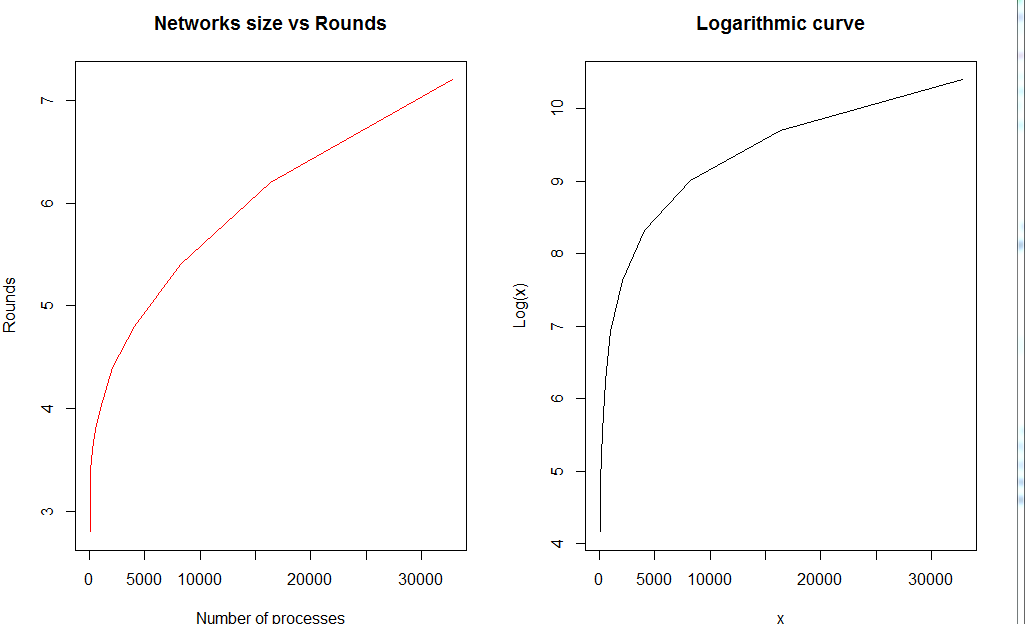
\includegraphics[width=1 \linewidth, height=6cm]{number_rounds.png} 
\caption{Rounds per execution vs log(x) curve}
\label{fig:rounds_execution}
\end{figure}



\begin{figure}[ht]
\centering
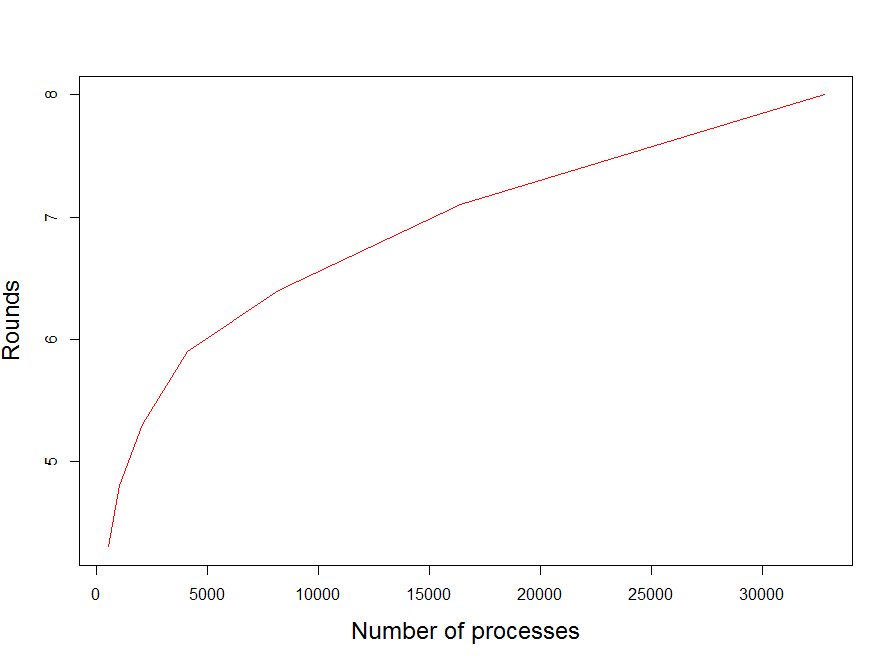
\includegraphics[width=1 \linewidth, height=8cm]{execution-rounds-erdos.PNG} 
\caption{Rounds of MIS algorithm using Erdos-Renyi model for network topologies}
\label{fig:rounds-erdos}
\end{figure}


It is expected that in each round of the algorithm some processes finish the local algorithm and become inactive until there are no more active processes, according to the proof of termination \cite{yves2009optimal}. This progression for a network of 32768 processes can be seen in the figure \ref{fig:progression}. The blue line represents the number of processes that join the \textit{MIS}  per round and the red line represents the processes that finish the algorithm but are not in the \textit{MIS}. The figure \ref{fig:actives}, shows the total number of processes that are active in each round for the same execution. In this example, by the end of round 14, the network has no active processes.  

\begin{figure}[ht]
\centering
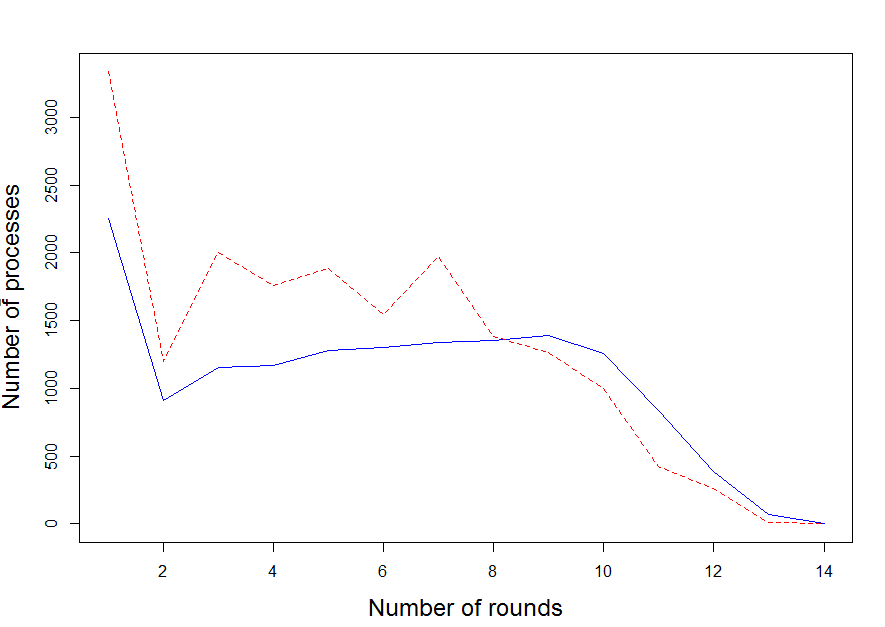
\includegraphics[width=1 \linewidth, height=8cm]{progress.PNG} 
\caption{Numbers of processes that finish the execution per round (in MIS and out of MIS)}
\label{fig:progression}
\end{figure}

\begin{figure}[bt]
\centering
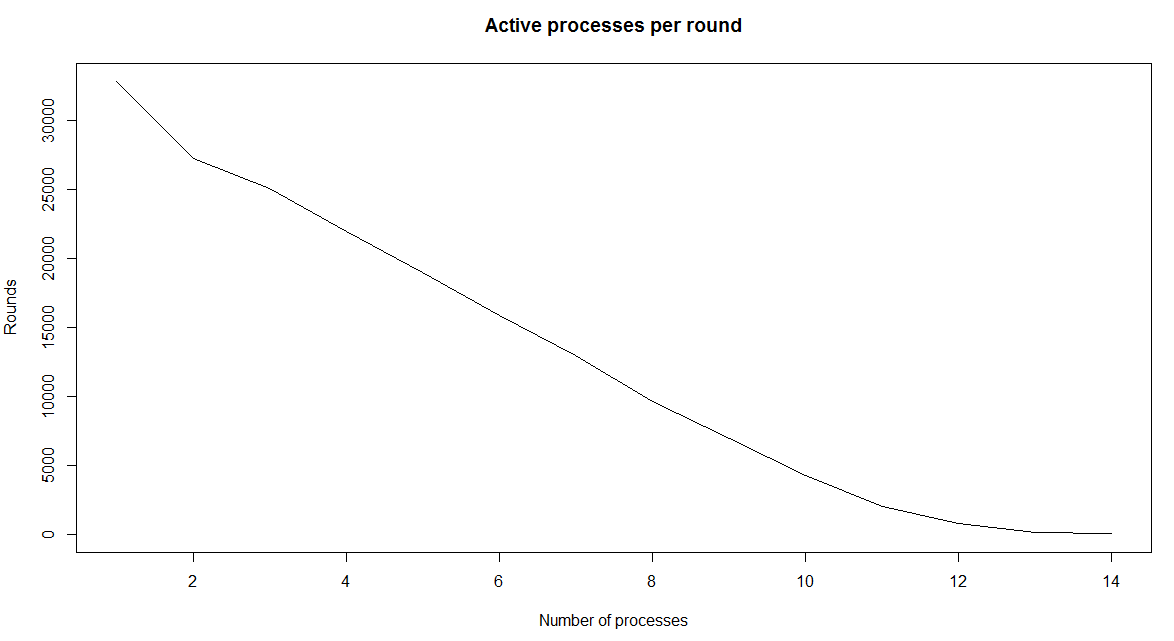
\includegraphics[width=1 \linewidth, height=7cm]{actives_round.PNG} 
\caption{Active processes per round}
\label{fig:actives}
\end{figure}

The analysis of the variation of the diameter of the graphs components was done on graphs with 32768 vertices and around 500000 edges on average. Initially, the graph consists of one connected component. The edges were generated according to the \textbf{SBM} and the values of parameters explained in the previous section. The diameters of the generated graphs before executing the algorithm were between 8 and 10. The figure \ref{fig:components_rounds} shows the average number of components of the graph for each round. The graphic shows a dramatic change in the number of components per round. The change always reaches its peak between the round two and four. This peak is also seen in the figure \ref{fig:diameter}, in which each point represents the diameter of one component of the graph. The same pattern is repeated in all executions, after the first round the graph is divided into one big component and a bunch of small components. In the following rounds, the size of the diameter of big component increases approximately between 25 and 40 and after the fourth round decrease dramatically again. Occasionally, it is formed components of diameter between 8 and 15. The relatively small diameter of the original graphs with respect to the size of the graph indicates a small average path length.  The increase in the diameter of the components was also observed in the tests executed on graphs generated with the Erd\~os--R\'enyi model. However, the number of vertices of the components were slightly lower, so does the diameter of the big component. Finally, around 30 \% of the vertices are part of the maximal independent set for both network models.  


\begin{figure}[ht]
\centering
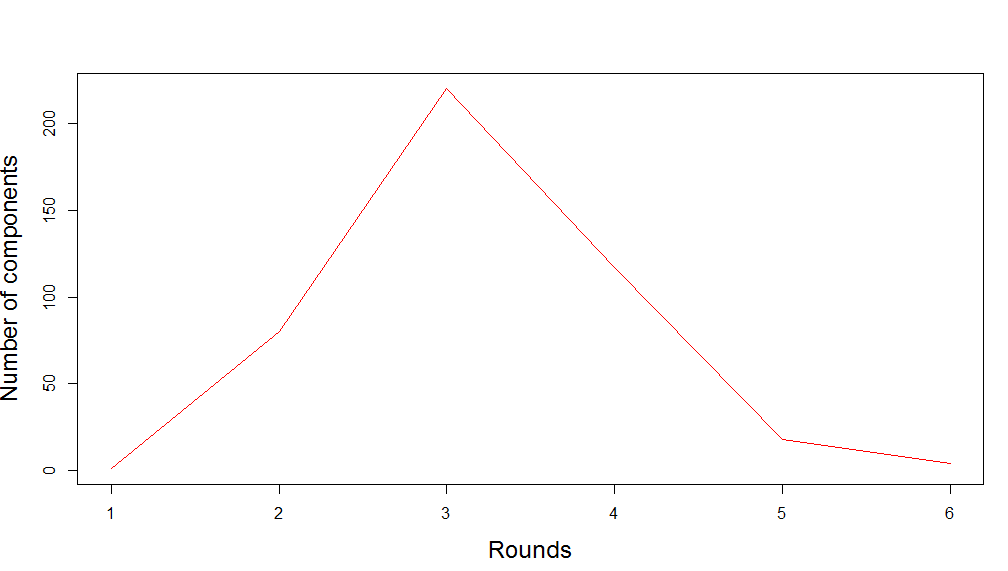
\includegraphics[width=1 \linewidth, height=8cm]{componentsVSrounds.PNG} 
\caption{Numbers of connected components per round}
\label{fig:components_rounds}
\end{figure}


\begin{figure}[htb]
\centering
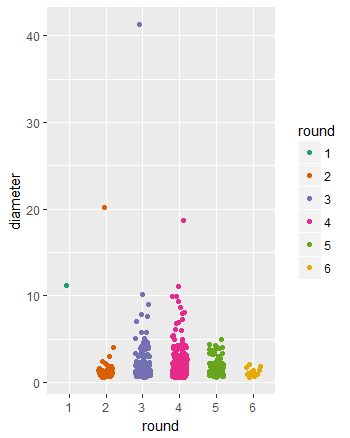
\includegraphics[width=1 \linewidth, height=16cm]{diameterSBM2.png} 
\caption{Diameter of connected components per round}
\label{fig:diameter}
\end{figure}

% \begin{figure}[ht]
% \centering
% \includegraphics[width=1 \linewidth, height=17cm]{mismember.PNG} 
% \caption{Number of vertices in the \textit{MIS}}
% \label{fig:mismember}
% \end{figure}

\FloatBarrier
\subsection{Evaluation of Synchronizers}

To evaluate the messages send by the algorithm, we need to make a distinction between messages sent by the synchronous algorithm and the additional messages sent by the synchronizers. In the case of Alpha and Beta, it is straightforward to count this two types of messages. Every time a process use the \textbf{sync-send} function, it is count as one message sent by the algorithm. For every synchronous message, the synchronizer sends some asynchronous messages according to its neighbourhood and the mechanism used to detect when a process is safe. For the Global synchronizer, the counting is a little more complicated. The messages for acknowledgement, for updating the topology and the notifications to the master process count as synchronisation overhead.


The figure \ref{fig:total_msg} illustrate the messages send by each synchronizer for the network of 32768 processes. The orange bar represents the synchronisation overhead and the blue bar the messages sent by the synchronous algorithm. It is clear that the global synchronizer is the one with the best performance. In this case, the synchronisation adds around $20 \%$ more messages. For the other two, the difference is overwhelming. The reason is that the Global synchronizer is optimal concerning the messages sent by active processes. In each round, once a process becomes inactive, no additional messages are sent by this process. On the contrary, Alpha and Beta require the entire topology to participate in every round until the distributed algorithm end.  

The figure \ref{fig:total_msg-round} shows how the number of messages decreases in each round for the global synchronizer, however, for Alpha and Beta remain constant. Finally, the figure \ref{fig:total_msg-size} shows the total number of messages send by the algorithm for different networks size. The messages complexity is bounded by the number of edges of the topology and a constant factor. The three functions show an approximate linear shape in agreement with the theoretical bounds.

\begin{figure}[ht]
\centering
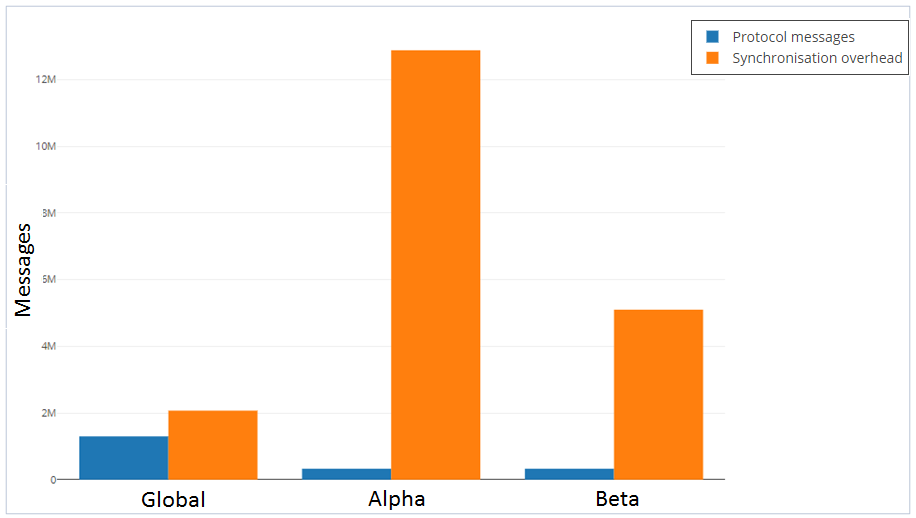
\includegraphics[width=1 \linewidth, height=7cm]{messages-synchroniser1.PNG} 
\caption{Messages send by the algorithm and Synchronizer}
\label{fig:total_msg}
\end{figure}

\begin{figure}[ht]
\centering
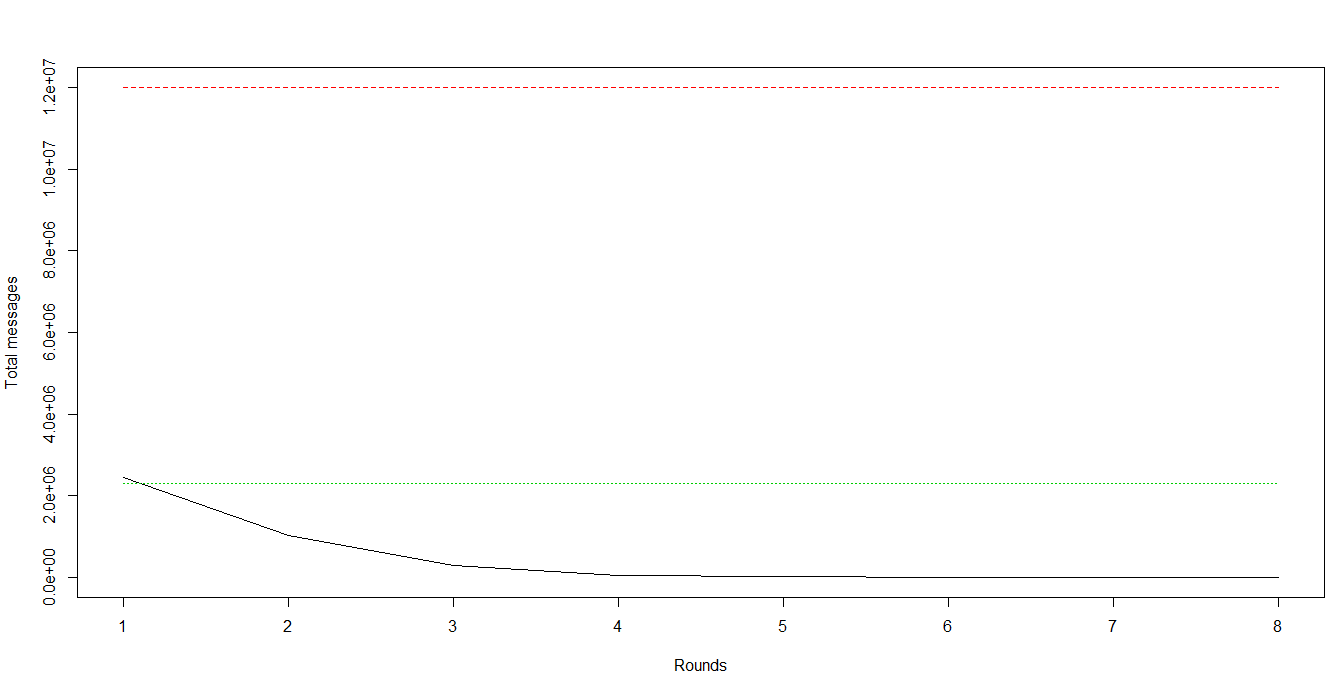
\includegraphics[width=0.9 \linewidth, height=8cm]{messages-rounds.PNG} 
\caption{Messages send by the algorithm in different rounds}
\label{fig:total_msg-round}
\end{figure}

\begin{figure}[ht]
\centering
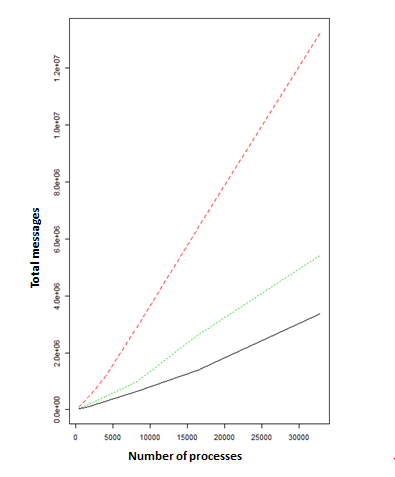
\includegraphics[width=1 \linewidth, height=14cm]{total_messages1.PNG} 
\caption{Total Messages vs Network size}
\label{fig:total_msg-size}
\end{figure}

\FloatBarrier
\subsection{Conclusions}

This dissertation focused on the problem of finding the Maximal Independent Set in general graphs. Distributed algorithms provide better time complexity than sequential algorithms for this problem.  The algorithm \ref{algorithm:main-mis}, proposed in \cite{yves2009optimal}, was implemented to analyse time and message complexity for the \textit{MIS} problem. Synchronous algorithms are easy to design and have lower complexity than the asynchronous counterpart. However, implement algorithms in a synchronous system requires extra messages to keep the processes synchronised in rounds. Two synchronizers using the local model were used to simulate synchronous communication: \textbf{Alpha} and \textbf{Beta} \cite{awerbuch1985complexity}.  A different approach is a global synchronizer based on a master process that controls the beginning and end of rounds. The global synchronizer was adapted to dynamic graphs, in which only active processes send messages and every process can communicate with a master processes. On the contrary, the local model is based only on communication between processes that share a communication channel. The \textit{MIS} algorithm and synchronizers were evaluated in time and message complexity. Additionally, an analysis of the changes of the graphs in different rounds and the size of the solution is presented. 

The experimental results show that the number of rounds that takes the algorithm \ref{algorithm:main-mis} to find the \textit{MIS} is consistent with the theoretical bound of $O(\log N)$. For the graph of 32768 vertices, it takes on average 10 rounds (as expected) to finish the algorithm. The extreme values are between 8 and 14 rounds for graphs generated with the \textbf{SBM} and the Erd\~os--R\'enyi model.  


The percentage of vertices which are in the \textit{MIS} is between 28 and 35 \%. There is no a constant rate in which the nodes or edges are removed from the graph. However, the half of the edges are removed in each phase in expectation \cite{yves2009optimal}. The empirical analysis of the diameter of the components suggests that edges are removed rapidly. In the first rounds, the graph is decomposed into one big component and a bunch of small components. The small components are eliminated from the graph almost immediately. Initially, the shortest path between any two vertices is small. However, as rounds are executed, edges are quickly removed and the diameter of the big component increase in factor between 2 and 5 until round 4 where start to decrease again. This increase can be produced because many edges are removed and it is harder to find short paths between vertices.  

Regarding the synchronizers, it is clear that the global synchronizer achieves the best performance in messages sent across the network. The extra step to calculate the active processes before each round provide a huge improvement in the performance because only actives processes send messages in each round. The drawback of the global synchronizer is that assumes that each process can send messages to the master process while in Alpha and Beta the communication is only between neighbours. Besides that, the master process becomes a bottleneck in the network. However, no practical issues in performance were observed in the simulation, even for the biggest graph of 32768 vertices. The trade-off between Alpha and Beta is on time and message. While Alpha perform has a good performance on time, Beta is better on message complexity. In practice, Alpha send more than the double of messages than Beta. For instance, for the 32768 network, Alpha send around 12 million messages in 14 rounds while Beta send around 5 million. The message complexity of the initialisation of Beta is in the order of $O(E)$. For the previous example, around 500000 extra messages are needed, which it is still much better than Alpha. Beta synchronizer requires a time overhead that is proportional to the height of the spanning tree, which is $O(V)$ in the worst case. However, in the simulation, the height was much lower, and there was no a significant difference between the time execution of the simulation with Alpha and Beta. So, in this case, Beta provides better performance in overall than Alpha if the local model is assumed.

An interesting extension of this project can be to analyse the properties of the algorithm with different types of network. Even if two models for random graphs were used, the diameter of components and number of vertices in the \textit{MIS} show the same pattern.  For the Erd\~os--R\'enyi model the edges have a uniform distribution, in the \textbf{SBM} the probability was equal for values out and inside of the diagonal but equals among them. Different grouping criteria using different probabilities for each block can be used to reach a more trusting conclusion.







\newpage
